\section{WIFI}
	Faire un réseau une seul cellule sur lequel les utilisateurs sont séparés en fréquences (FDMA). Bande wifi autour 2.4Ghz avec 14 bande 5Mhz avec un débit de 1 a 11MB/s
	\subsection{Modulation}
		Se fait en \textbf{DSSS}, aujourd’hui les nouveaux standards remplacent DSSS par OFDM. DSSS utilise du CDMA et possède une largeur de bande de 22Mhz, cette largeur couvre plusieurs canaux.
		
		Les nouveaux standards OFDM utilisent une sorte de FDMA. La bande est divisée en beaucoup de petites sous-bandes qui sont rendues indépendantes par le traitement du signal. Ce qui a un énorme impact sur la bande passante
		
		Le standard du futur est le MIMO (multiple input multiple output). Cette technique utilise plusieurs antennes en même temps. Ce standard lève 3 soucis de design :
		
		\begin{itemize}
			\item Beamforming : Le standard du futur est le MIMO (multiple input multiple output). Cette technique utilise plusieurs antennesen même temps. Ce standard lève 3 soucis de design :
			\item Multiplexage spatial : Les messages divisé doivent être réassemblé pour récuperer le canal sur lequel transite les données. 
			
				\begin{figure}[H]
					\centering
					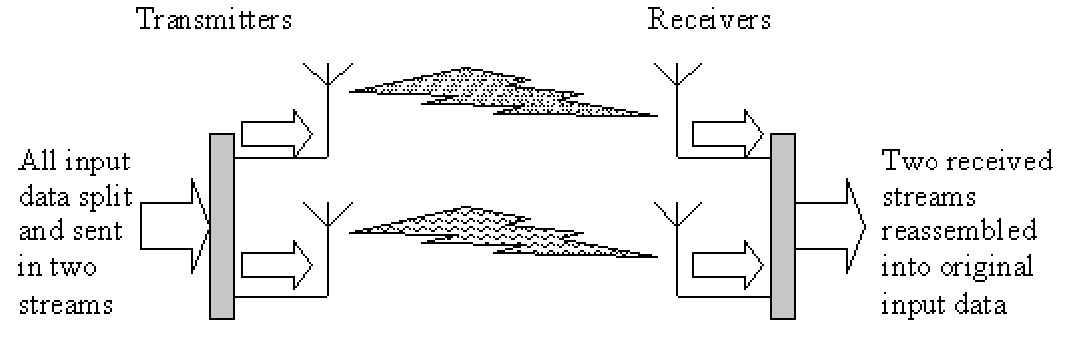
\includegraphics[width=\textwidth]{img/wifi/M.png}
				\end{figure}
			\item Conbattre les évanouissement : La réception peut varier énormément d’un endroit à un autre. Comme il y a plusieurs antenne envoyant un signal il y a la possiblité qu’un signal arrive et l’on choisis le meilleur signal arrivant. Il faut évidemement que les antennes soit suffisement espacé (Au moins $\lambda$/2 ).
On lutte donc contre les trajets multiples !
		\end{itemize}
		
	\subsection{Standard}
		\begin{figure}[H]
			\centering
			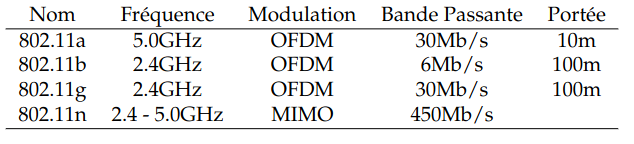
\includegraphics[width=\textwidth]{img/wifi/S.png}
		\end{figure}
		